\documentclass[11pt,oneside]{book}
\usepackage[margin=1.2in]{geometry}
\usepackage[
    backend=biber,
    style=numeric,
    giveninits=true
]{biblatex}
\usepackage{ragged2e}
\usepackage{setspace}
\usepackage[toc,page]{appendix}
\usepackage[none]{hyphenat}
\usepackage{graphicx}
\usepackage{tikz}
\usepackage{makecell}

\usetikzlibrary{shapes.geometric, positioning, fit}
\addbibresource{bibliography.bib}

% Literature bibliography style
\defbibenvironment{nolabelbib}
  {\list
     {}
     {\setlength{\leftmargin}{\bibhang}%
      \setlength{\itemindent}{-\leftmargin}%
      \setlength{\itemsep}{\bibitemsep}%
      \setlength{\parsep}{\bibparsep}}}
  {\endlist}
  {\item}

% Easy citation command
\newcommand{\ccite}[2]{#1\textsuperscript{\cite{#2}}}

\begin{document}

\frontmatter

\begin{titlepage}
    \begin{center}
        
\includegraphics[width=5cm]{images/UOSLogo_Portrait_Violet_RGB.png}\\[2cm]
        \linespread{1.2}\huge Description Report: {\bfseries Evolutionary Optimization of Quantum Circuits for Automated Circuit Design}\\[2cm]
        \linespread{1}
        {\Large Eryk Arkadiusz Majoch}\\[1cm]
        {\large \emph{Supervisor:} Phil McMinn}\\[1cm]
        \large COM3610 \\
        \today
    \end{center}
\end{titlepage}

\newpage
\tableofcontents

\setstretch{1.1} 

\mainmatter
\chapter{Introduction}
\section{Background}

Quantum computing stands at the forefront of technological innovation, promising to revolutionise fields such as cryptography and drug discovery. Quantum computing leverages the principles of quantum mechanics to perform computations that would not be feasible for classical computers. By utilising quantum properties such as superposition and entanglement, quantum computers have the potential to solve certain problems much faster than their classical \ccite{counterparts}{10062753}.

However, the design of effective quantum circuits remains a significant challenge, often requiring experience in both quantum mechanics and computer science. Quantum circuits, the basis of quantum algorithms, consist of a series of quantum gates applied to qubits, manipulating quantum states to perform \ccite{computations}{wong2022introduction}. Traditional approaches to quantum circuit design rely heavily on human intuition and deep knowledge, which can be an obstacle in the development of new quantum algorithms.

Platforms like IBM's \ccite{Quantum Composer}{ibmcomposer} have made it easier for researchers to manually create quantum circuits. However, as the complexity of quantum algorithms grows, manual design becomes increasingly difficult and time consuming. This limitation highlights the need for automated approaches to quantum circuit design.

\section{Aims and Objectives}

This project aims to address the challenges of manual quantum circuit creation by exploring the application of Genetic Programming (GP) to automate the design process. GP, a subset of evolutionary algorithms, offers a promising approach to automated program \ccite{synthesis}{10.1007/978-3-031-42441-0_8}, evolving computer programs by applying principles inspired by biological evolution.

The primary objectives of this project are:
\begin{itemize}
    \item Develop a complete simulation environment for quantum circuits using genetic programming
    \item Define appropriate genetic operations for circuit evolution
    \item Define fitness functions that guide the evolution process towards the desired circuit behaviour
    \item Analyse the effectiveness of evolutionary optimisation for quantum circuits by comparing them to already existing solutions using publicly available benchmarks
\end{itemize}

To ensure the quality and usability of the resulting simulation environment, it is essential to define key characteristics that must be followed:
\begin{itemize}
    \item \textbf{Simplicity}: The platform should be easily configurable for the end user, with clear parameters and intuitive interfaces.
    \item \textbf{Clear Output}: The platform should generate its output in a preferably standardised format, ensuring that users can easily read, understand, and potentially integrate the results with other tools.
    \item \textbf{Performance}: The platform should demonstrate reasonable computational efficiency.
    \item \textbf{Scalability}: The platform should be designed to run both locally on classical computers and on High Performance Computing (HPC) clusters, allowing for the evolution of more complex quantum circuits when greater computational resources are available.
\end{itemize}

\section{Studied Literature}

\nocite{*}
\printbibliography[env=nolabelbib, keyword={lit}, heading=none]

% Chapter word count: 399

\chapter{Analysis}
\section{Problem Decomposition}

The task of optimising automated quantum circuit design can be decomposed into three main categories:
\begin{enumerate}
    \item \textbf{Genetic Programming Algorithm}
    \item \textbf{Information Representation}
    \item \textbf{Simulation Program}
\end{enumerate}

Each of these categories presents unique challenges that need to be addressed to achieve the desired outcome. All the identified challenges also contain possible solutions which will be considered in the final solution and explained in a later section of the dissertation. They'll be experimented on or combined in order to see which yield the best possible outcomes. This is only an initial proposal of possible solutions as more may arise through further research if generated results aren't of expected quality.

\subsection{Genetic Programming Algorithm}
Genetic programming frameworks allow us to control every step of the evolution procedure. With this, we are able to tailor the framework to our needs. Here are the key aspects which will be fine-tuned as a part of this projects research:

\begin{table}[h!]
    \centering
    \setlength\tabcolsep{0pt}
    \begin{tabular*}{\linewidth}{@{\extracolsep{\fill}}|c|c|c|c|} 
        \hline
        \textbf{Fitness Functions} & \textbf{Selection Methods} & \textbf{Crossover Methods} & \textbf{Mutation Methods} \\ \hline
        Fidelity Function & Random Selection & Single-point Crossover & Single Gate Flip \\ [1ex]
        Entanglement Function & Tournament Selection & Multi-point Crossover & Mutate Qubits \\ [1ex]
         &  &  & Mutate Gates \\ [1ex]
        \hline
    \end{tabular*}
    \caption{Genetic Algorithm Decomposition Table}
\end{table}


\subsection{Information Representation}
The next significant problem concerns the representation of any data stored within the program. There needs to be a way for the user to provide their circuit requirements in a simple way when using the program. During the evolutionary process, the circuits must be represented in such way that the algorithm may perform its steps comfortably. When simulation has finished, it would be preferable to use a standardised format whilst exporting the generated circuit in order to keep the possibility of using them with other tools open.

\begin{table}[h!]
    \centering
    \begin{tabular}{|c|c|c|c|} 
        \hline
        \textbf{User's Description} & \textbf{Circuit Representation} & \textbf{Output Generation} \\ \hline
        Unitary Matrix & String Encoding & Visual Circuit Diagram \\ [1ex]
        Truth Table & Directed Acyclic Graph & Qiskit Class Instance \\ [1ex]
        Circuit Properties & Quantum Assembly Language & \\ [1ex]
        \hline
    \end{tabular}
    \caption{Information Representation Decomposition Table}
\end{table}

\subsection{Simulation Program}
The final significant consideration is the user's interaction with the program itself. The simulation environment needs to be versatile by allowing the user to configure all of their requirements as well as be user-friendly.

\begin{table}[h!]
    \centering
    \begin{tabular}{|c|c|c|c|} 
        \hline
        \textbf{Interface} & \textbf{Scalability} \\ \hline
        Command Line Interface (CLI) & Local execution on personal computers \\ [1ex]
        Graphical User Interface (GUI) & \makecell{Distributed execution on\\High Performance Computing (HPC) clusters} \\ [1ex]
        \hline
    \end{tabular}
    \caption{Simulation Program Decomposition Table}
\end{table}

\section{Proposed Technologies}
To address these challenges I will be using the following technologies. The program will be written using the Python programming \ccite{language}{python} due to its popularity in machine learning tasks as well as extenisve availability of third-party frameworks. The genetic programming framework of choice is \ccite{PyGAD}{gad2023pygad} due to its customisability and for the GUI I've decided on \ccite{PyQt}{pyqt} due to my familiarity with its C++ library. I will also be using IBM's Qiskit quantum computing \ccite{framework}{qiskit} which is known for its representation, simulation and visualisation of quantum circuits. 

% Chapter word count: 359

\chapter{Plan of Action}
This project will take place over the whole span of this academic year with key milestones and deliverables planned to ensure steady progress and timely completion.

In the first semester, the focus will be on laying a solid foundation for the whole project. It will begin with extensive background reading on quantum computing and its applications. Concurrently, a literature survey will be conducted to dive deeper into the complicated process of optimising evolutionary quantum circuit design. This phase will also involve defining system requirements and conducting an analysis of the problem space.

After the first couple weeks, the project will enter its initial implementation stage where the basic GP framework alongside the quantum circuit simulation environments will be worked on. This will involve implementing basic genetic operations as well as establishing quantum circuit representation.

The second semester will primarily focus on optimisation of the GP algorithm. Rigorous testing and validation of the system will be conducted throughout this stage, as well as data collection for the final report. The final weeks will be devoted to documentation, result analysis and final report editing.

Throughout the duration of the project, regular meetings with my project supervisor will be scheduled in order to ensure the project will be completed on time and to address any issues or question that arise. The Gantt charts below provide a rough visual representation of the project timeline.

\begin{figure}[h!]
    \centering
    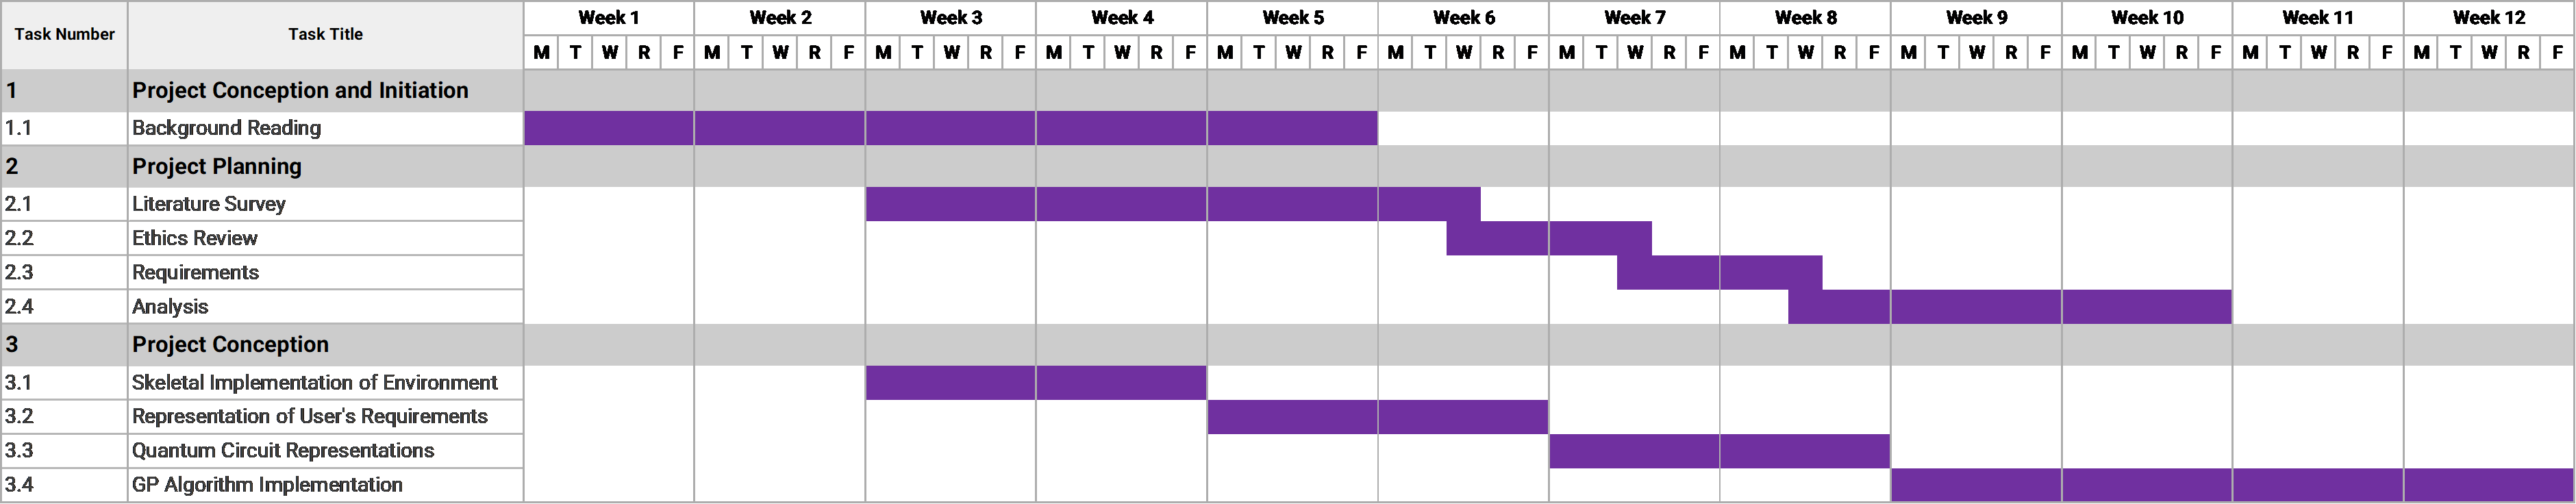
\includegraphics[width=\textwidth]{images/gantt_1.png}
    \caption{Gantt chart for semester one}
\end{figure}

\begin{figure}[t!]
    \centering
    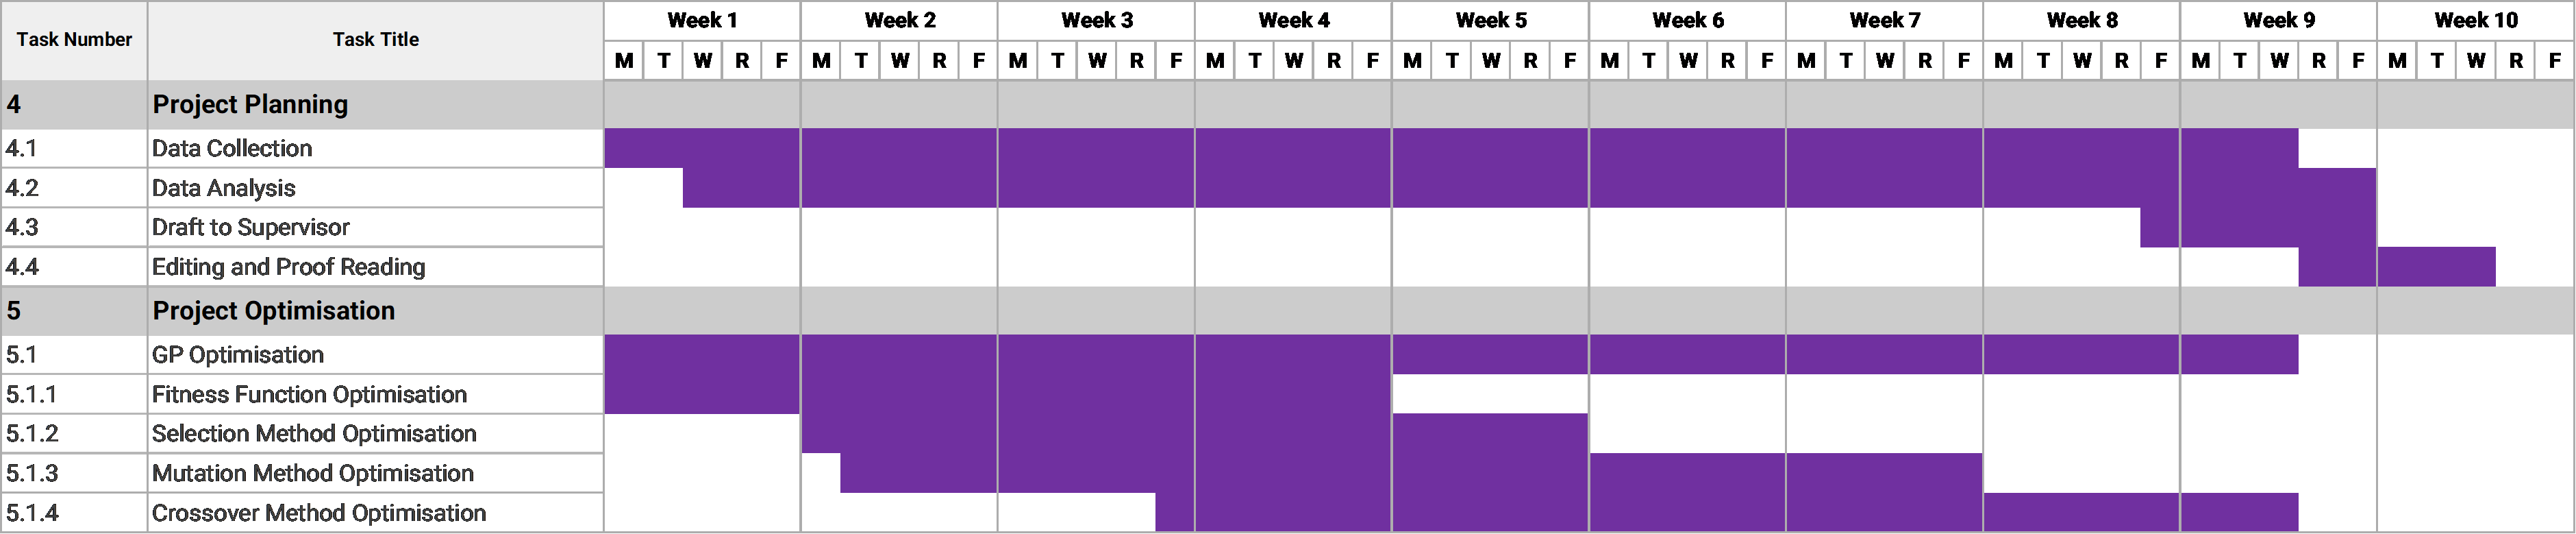
\includegraphics[width=\textwidth]{images/gantt_2.png}
    \caption{Gantt chart for semester two}
\end{figure}

% Chapter word count: 230


\printbibliography[notkeyword=lit]

\end{document}